\setlength{\footskip}{8mm}

\chapter{Introduction}

\section{Objectives}

The overall objective of the study report is to build an understanding of the tools and techniques of analytics used by financial analysts and institutions. This study presents a brief of the current state of affairs analytics and subsequently a study of the techniques. Also there is a demonstration of some common methods.


\section{Overview}

Data analysis is an very robust topic in the field of data science and encompasses the various mathematical functions. The functions are statistical in nature and are performed on the data obtained. The goal of data analytics is to support (or reject) the hypothesis which the data scientist postulates.
“ By processing a steady stream of real-time data, organizations can make time-sensitive decisions faster than ever before, monitor emerging trends, course-correct rapidly and jump on new business opportunities.” [BIG Data Analytics: A Framework for Unstructured Data Analysis pdf]

This paper tries to enlist most of the up-to-date techniques used by researchers and mathematicians to make sense of the data. Also the paper presents them in three groups of analytics.
But then there arises a question which is, why the need for data analytics ? Well, to answer that the paper proposes the literature from an article of Kdnuggets \shortcite{KDnuggets}.



According to Paul following are use cases  of data analytics :
1. Analytics powers our decisions – we do not need to guess while making bold new decisions, we should use the information from data at hand.
2. Your data analysis weighs down your opponent's argument.
3. Cut down on loss making ventures with data analytics.
4. Can be applied to all domains be it health-care, banking, marketing, sales, operations etc.
On the scenario when describing Data analytics it is very important to put the focus on Hypothesis.

Shown in the table \ref{tableDMusecase} is some business areas 


\begin{table}[H]
	\centering
%	\hskip-1.8cm
	\begin{tabular}{|p{4cm}|p{4cm}|l|}
		\hline
		\textbf{Application area} & \textbf{Applications} & \textbf{Specifics}\\
		\hline
		Insurance & Fraud detection & Identify claims meriting investigation\\
		\hline
		Telecom & Churn & Identify likely customer turnover\\
		\hline
		Telemarketing & On-line information & Aid telemarketers with easy data access\\
		\hline
		Human resource management & Churn & Identify potential employee turnover\\
		\hline
		\multirow{2}{4em}{Retail}  & Affinity positioning & Position product effectively\\
		& Cross-selling & Find more products for customers\\
		\hline
		\multirow{2}{4em}{Banking} & Customer relationship management & Identify customer value\\
		&& Develop programs to maximize revenue\\
		\hline
		Credit card management & Lift & Identify effective market segments\\
		& Churn & Identify likely customer turnover\\
		\hline
	\end{tabular}
	\caption{Data mining use cases}
	\label{tableDMusecase}
\end{table}
	
Figure \ref{fig:data-analytics} is a view of the data analytics with respect to the main fields.

\begin{figure}[H]
	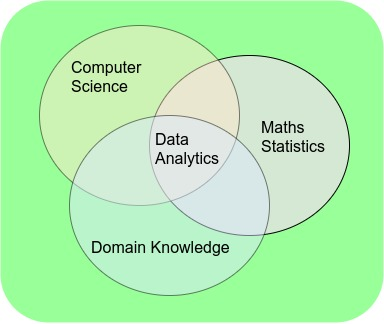
\includegraphics[scale = 0.8]{figures/FlowChart.jpg}
	\centering
	\caption{Data Analytics}
	\label{fig:data-analytics}
\end{figure}
\FloatBarrier

\newpage
\section{Why Analytics for financial institutions ?}
According to a joint research study, by Boston Consulting Group and Morgan Stanley with analytics professionals, it was reveled that the financial institutions lagged behind other verticals in the use of data analytics~\shortcite{BCGanalytics2017} and it is shown in figure~\ref{fig:da_digitization}. One of the findings of the research was that FI's are investing a lot of capital, an estimated total of about \textdollar1bn. In addition it was found that for near term value creation the FI's expected data analytics to optimize customer acquisition, customer retention, operational efficiency, and risk mitigation.
\newline
\newline
\begin{figure}[H]
	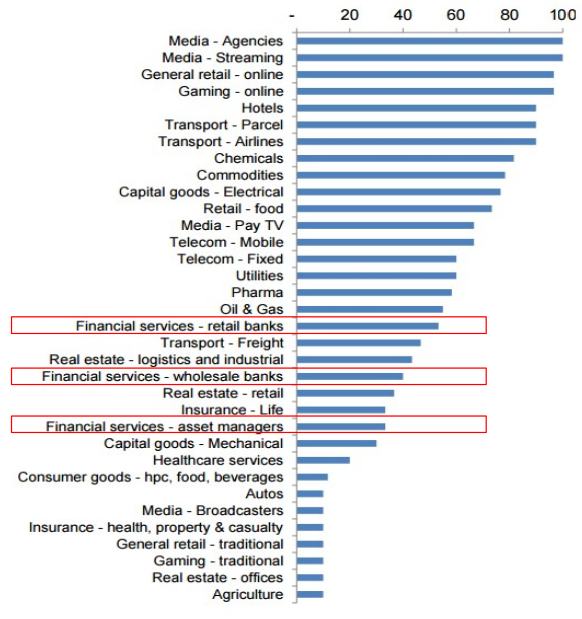
\includegraphics[scale = 0.7]{figures/DA_used_verticals.png}
	\caption{Reprinted from the Morgan Stanley Digitization Index ranks }
	\label{fig:da_digitization}
\end{figure}
\FloatBarrier

\newpage
\section{State of analytics in financial companies}
From the survey of FI's, a mix of interviewees representing payment companies, service providers, insurance, commercial banks, BCG made some interesting discoveries. It was found that most organizations have invested in analytics techniques to generate market perceptions. Some of the most used were those of social media, log, text and location analytics as shown in figure~\ref{fig:da_capabilities}.

\begin{figure}[H]
	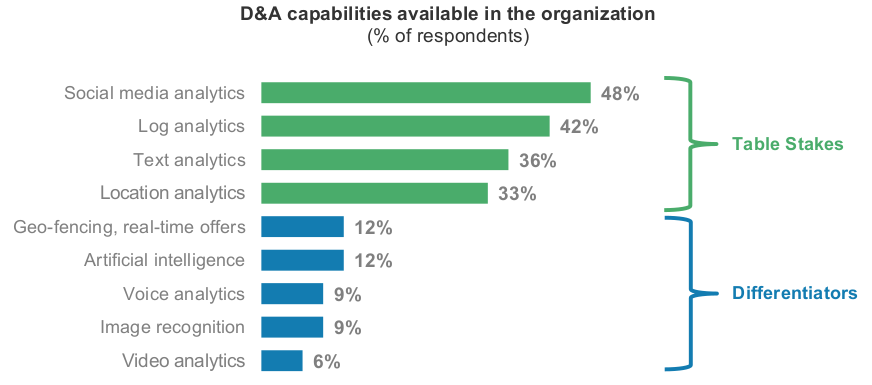
\includegraphics[scale = 0.5]{figures/DA_capabilities.png}
	\caption[Da capablities]{Reprinted from the work of Boston consulting group  }
	\label{fig:da_capabilities}
\end{figure}
\FloatBarrier

Researchers have highlighted that most of the interviewees claimed that institutions are yet to make substantial gain from investments in analytics. They identified that companies can make gains from automation and digitization of manual processes. Additionally, it was noted that financial institutions are adopting digital processes to automate data collection for KYC (Know Your Customer) service and Anti-money laundering 
%\newline
%\newline
Customers are loyal consumers of products, which give value for their monetary investments. Big institutions tend to over look the need for value creation and focus their analytics and metrics to improve profit \shortcite{Reichheld1996}. In the HBR report Reichheld makes certain  observations that customers of large companies witness degrading value standards and secondly increasing rate of customer churn is a good variable to predict cash flow from consumer to company. He also noted that companies can replace old customer with new ones but the profits are lower as cost of induction is high.

